% Content for Chapter 5, Section 5.9 — pulled in by chapters/05-system-design.tex
\subsection{دور الخدمة ونطاقها}

تتابع هذه الخدمة الشرح أثناء الجلسة الحيّة، فتحوّل صوت المعلّم إلى نصّ، وتقارن ما يشرحه بالمادة المرجعية المفهرسة، وترسل إليه ملاحظة خاصّة عند رصد فرق أو نقص. وهي الخدمة الوحيدة التي يقوم مسارها الرئيس على حلقة مستمرّة تعمل طوال الجلسة، لا على دورة طلب وجواب.

\subsection{مكوّنات الخدمة}

تنتظم مكوّنات طبقة التطبيق مراحلَ متتابعة تمثّل هذه الحلقة: التقاط الصوت، وتحويله إلى نصّ، وكشف حدّ الفكرة، وتقييمها مقابل المصادر، وضبط إيقاع التدخّل، ثمّ إرساله. ويعرض الشكل~\ref{fig:comp-06} هذه المكوّنات وروابطها الخارجية.

% [H]: pinned under the paragraph that introduces it. At 2.09:1 full width is
% only ~32% of the text block, so it fits without shrinking.
\begin{figure}[H]
  \centering
  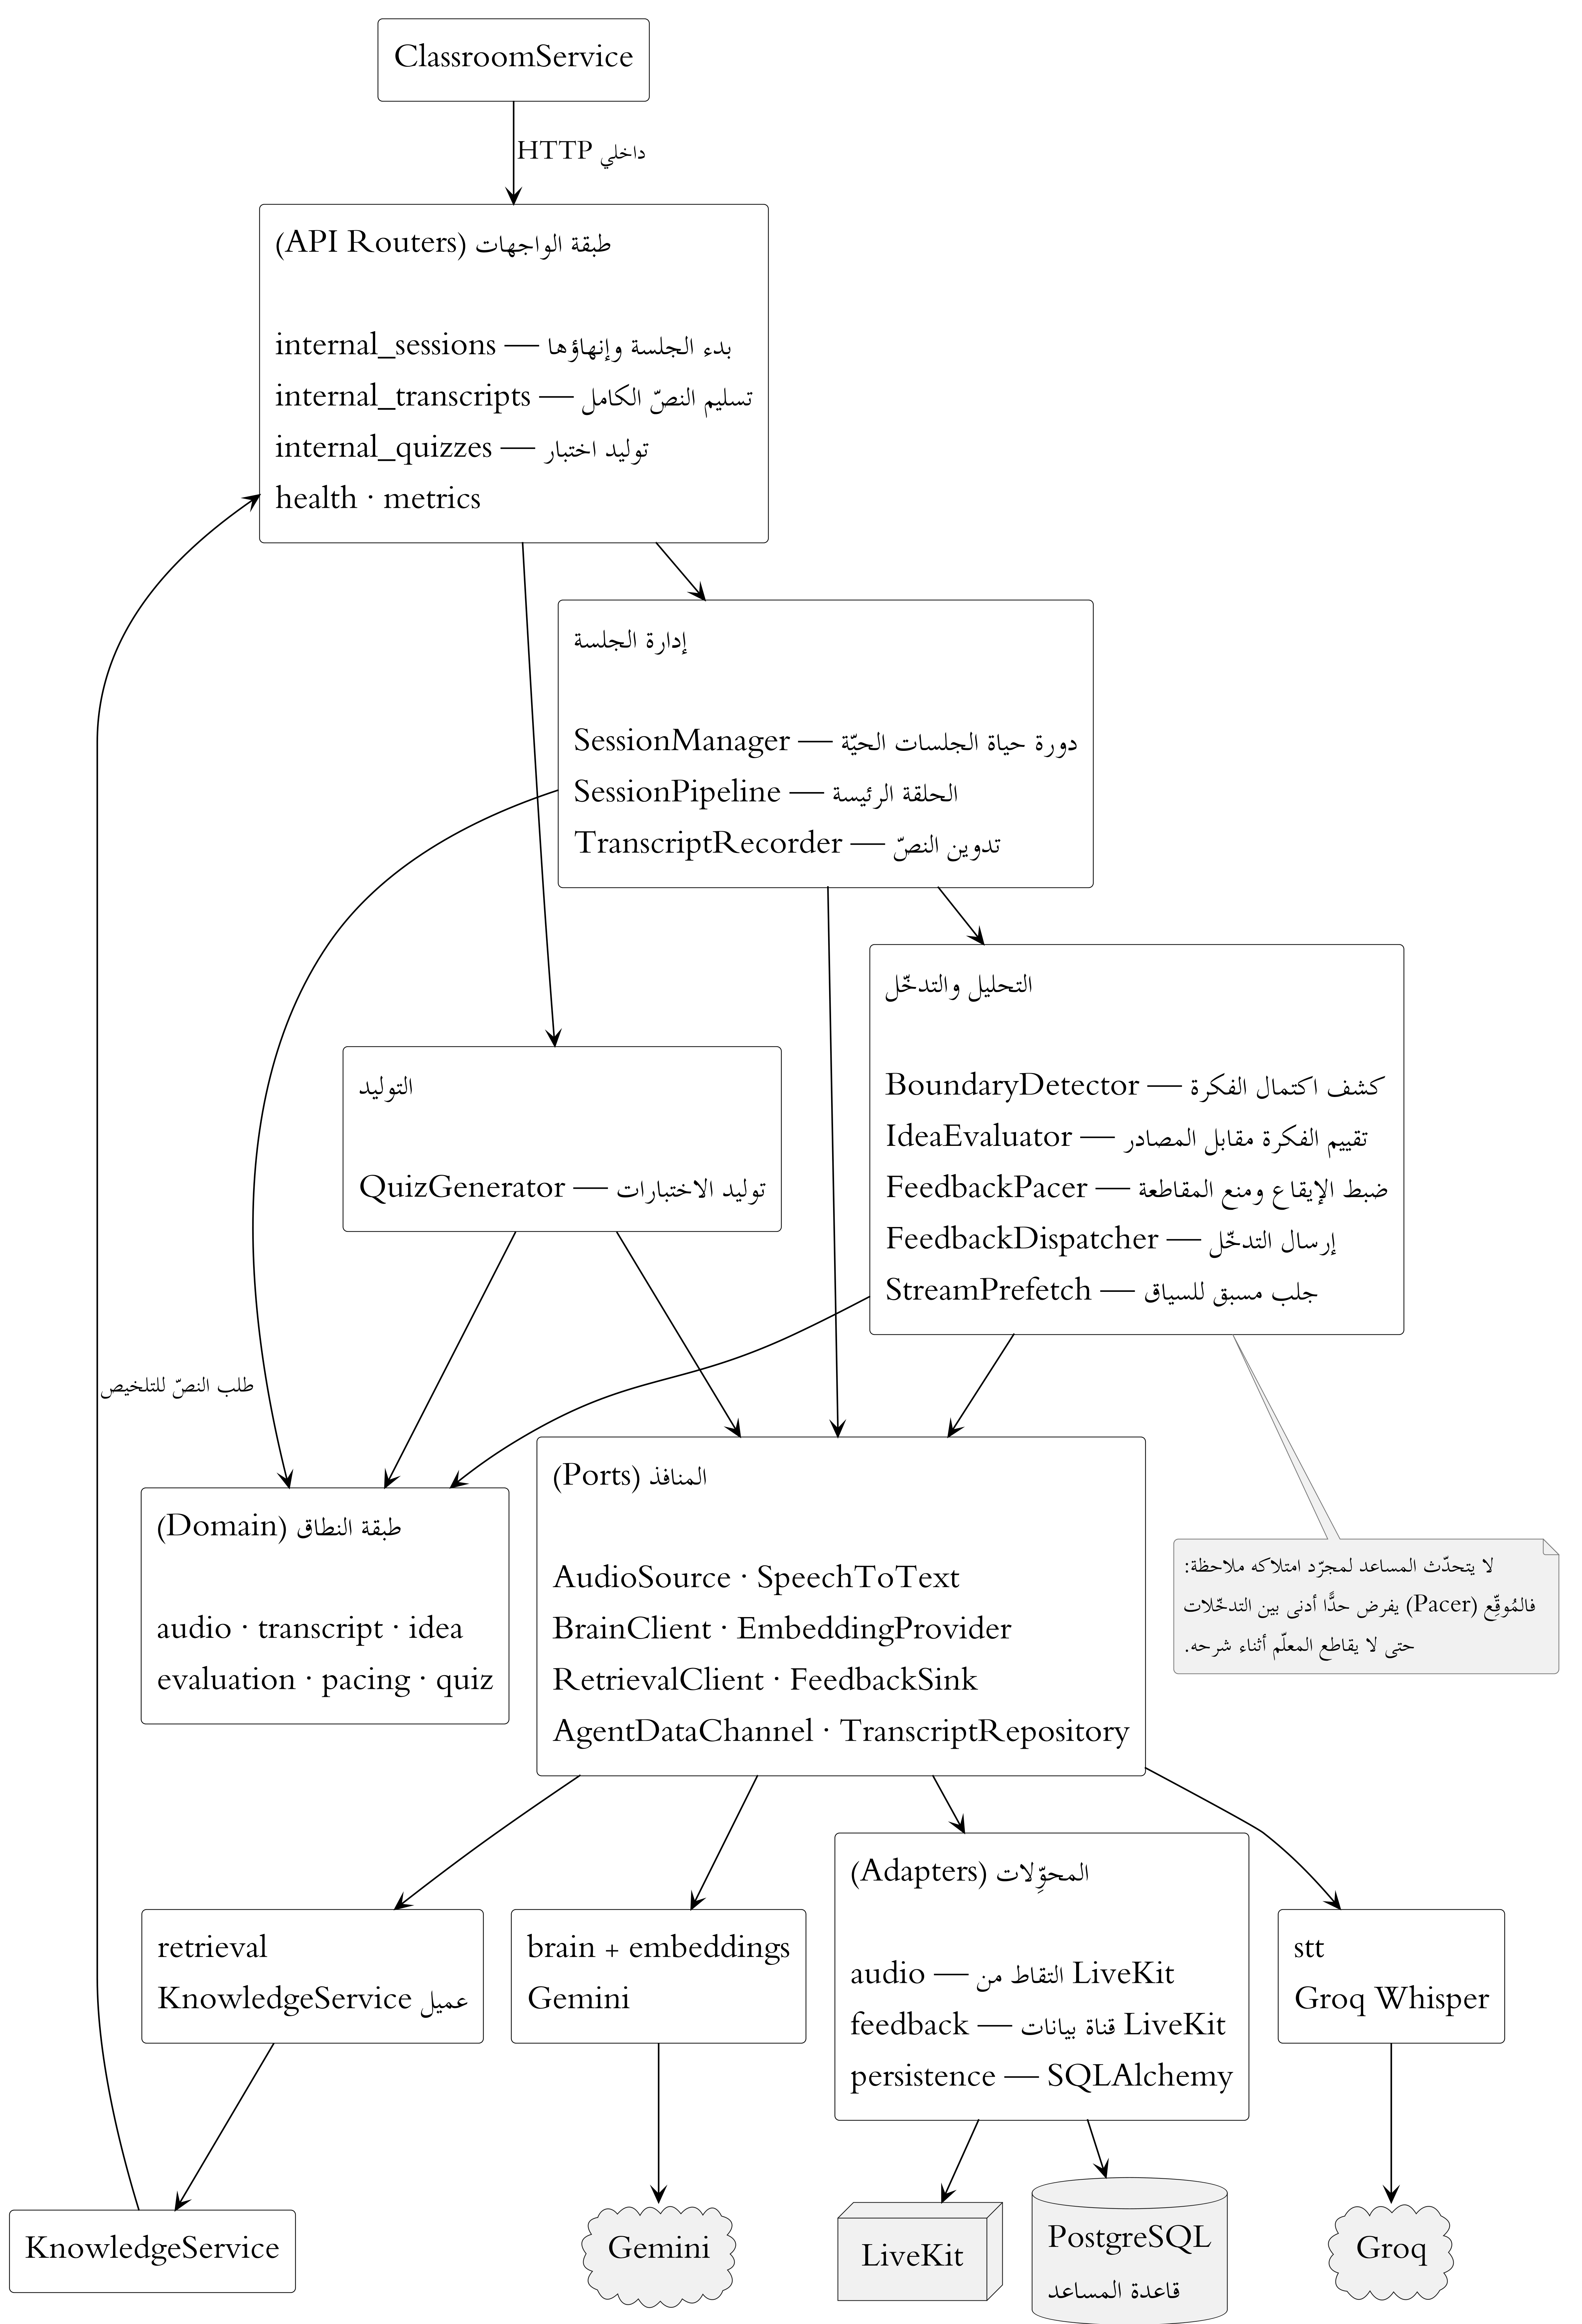
\includegraphics[width=\textwidth,height=0.8\textheight,keepaspectratio]{figures/comp-06-live-assistant.png}
  \caption{مخطط مكوّنات خدمة المساعد المباشر.}
  \label{fig:comp-06}
\end{figure}

وطُبّق في هذه الخدمة نمط المنافذ والمحوِّلات: يقابل كلَّ مورد خارجي منفذٌ مجرّد في طبقة التطبيق ومحوِّل واحد خلفه في طبقة البنية التحتية، وذلك لمصدر الصوت ومحرّك تحويل الكلام إلى نصّ والنموذج التوليدي ومزوّد التضمين وعميل الاسترجاع وقناة إرسال التدخّل ومستودع النصّ. ويتيح ذلك استبدال أيّ مزوّد دون تعديل منطق الحلقة، وتشغيل الحلقة كاملةً في الاختبارات بمحوِّلات بديلة لا تتّصل بشبكة.

وتحمل طبقة النطاق أنواع القرار نفسها: اكتمال الفكرة، ونتيجة التقييم ودرجة خطورتها، وقرار الإيقاع وسبب الكبح. وهي منطق خالص لا يستدعي نموذجًا ولا اتصالًا شبكيًّا ولا قاعدة بيانات، فتقبل الاختبار الوحدوي دون أيّ اعتماد خارجي.

ويفصل مُوقِّع التدخّل (\en{FeedbackPacer}) بين صحّة الملاحظة ووصولها إلى المعلّم، فيطبّق أربع قواعد بالترتيب، وتوقف أُولاها تحقّقًا الإرسالَ: حدّ أدنى لدرجة الثقة، وسقف لعدد التدخّلات في الجلسة الواحدة، وحدّ أدنى زمني بين تدخّلين متتاليين، ورفض الملاحظة المشابهة لما أُرسل ضمن نافذة زمنية محدّدة. والغرض منع مقاطعة المعلّم في أثناء الشرح.

وتُعرض الحلقة كاملةً، من التقاط الصوت إلى قرار التدخّل، في القسم~\ref{subsubsec:flow-live-loop}.

\subsection{نموذج البيانات}

لا تحفظ هذه الخدمة إلّا نصّ الجلسة؛ أمّا التسجيل والملخّص فيقعان في خدمة الفصول الدراسية ومخزن الملفّات. ويقوم النموذج على كيانين يعرضهما الشكل~\ref{fig:erd-05}: ترويسة النصّ (\en{session\_transcripts}) ومقاطعه المرتّبة زمنيًّا (\en{transcript\_segments}).

% [H]: pinned under the paragraph that introduces it. At 2.63:1 full width is
% only ~26% of the text block, so it fits without shrinking.
\begin{figure}[H]
  \centering
  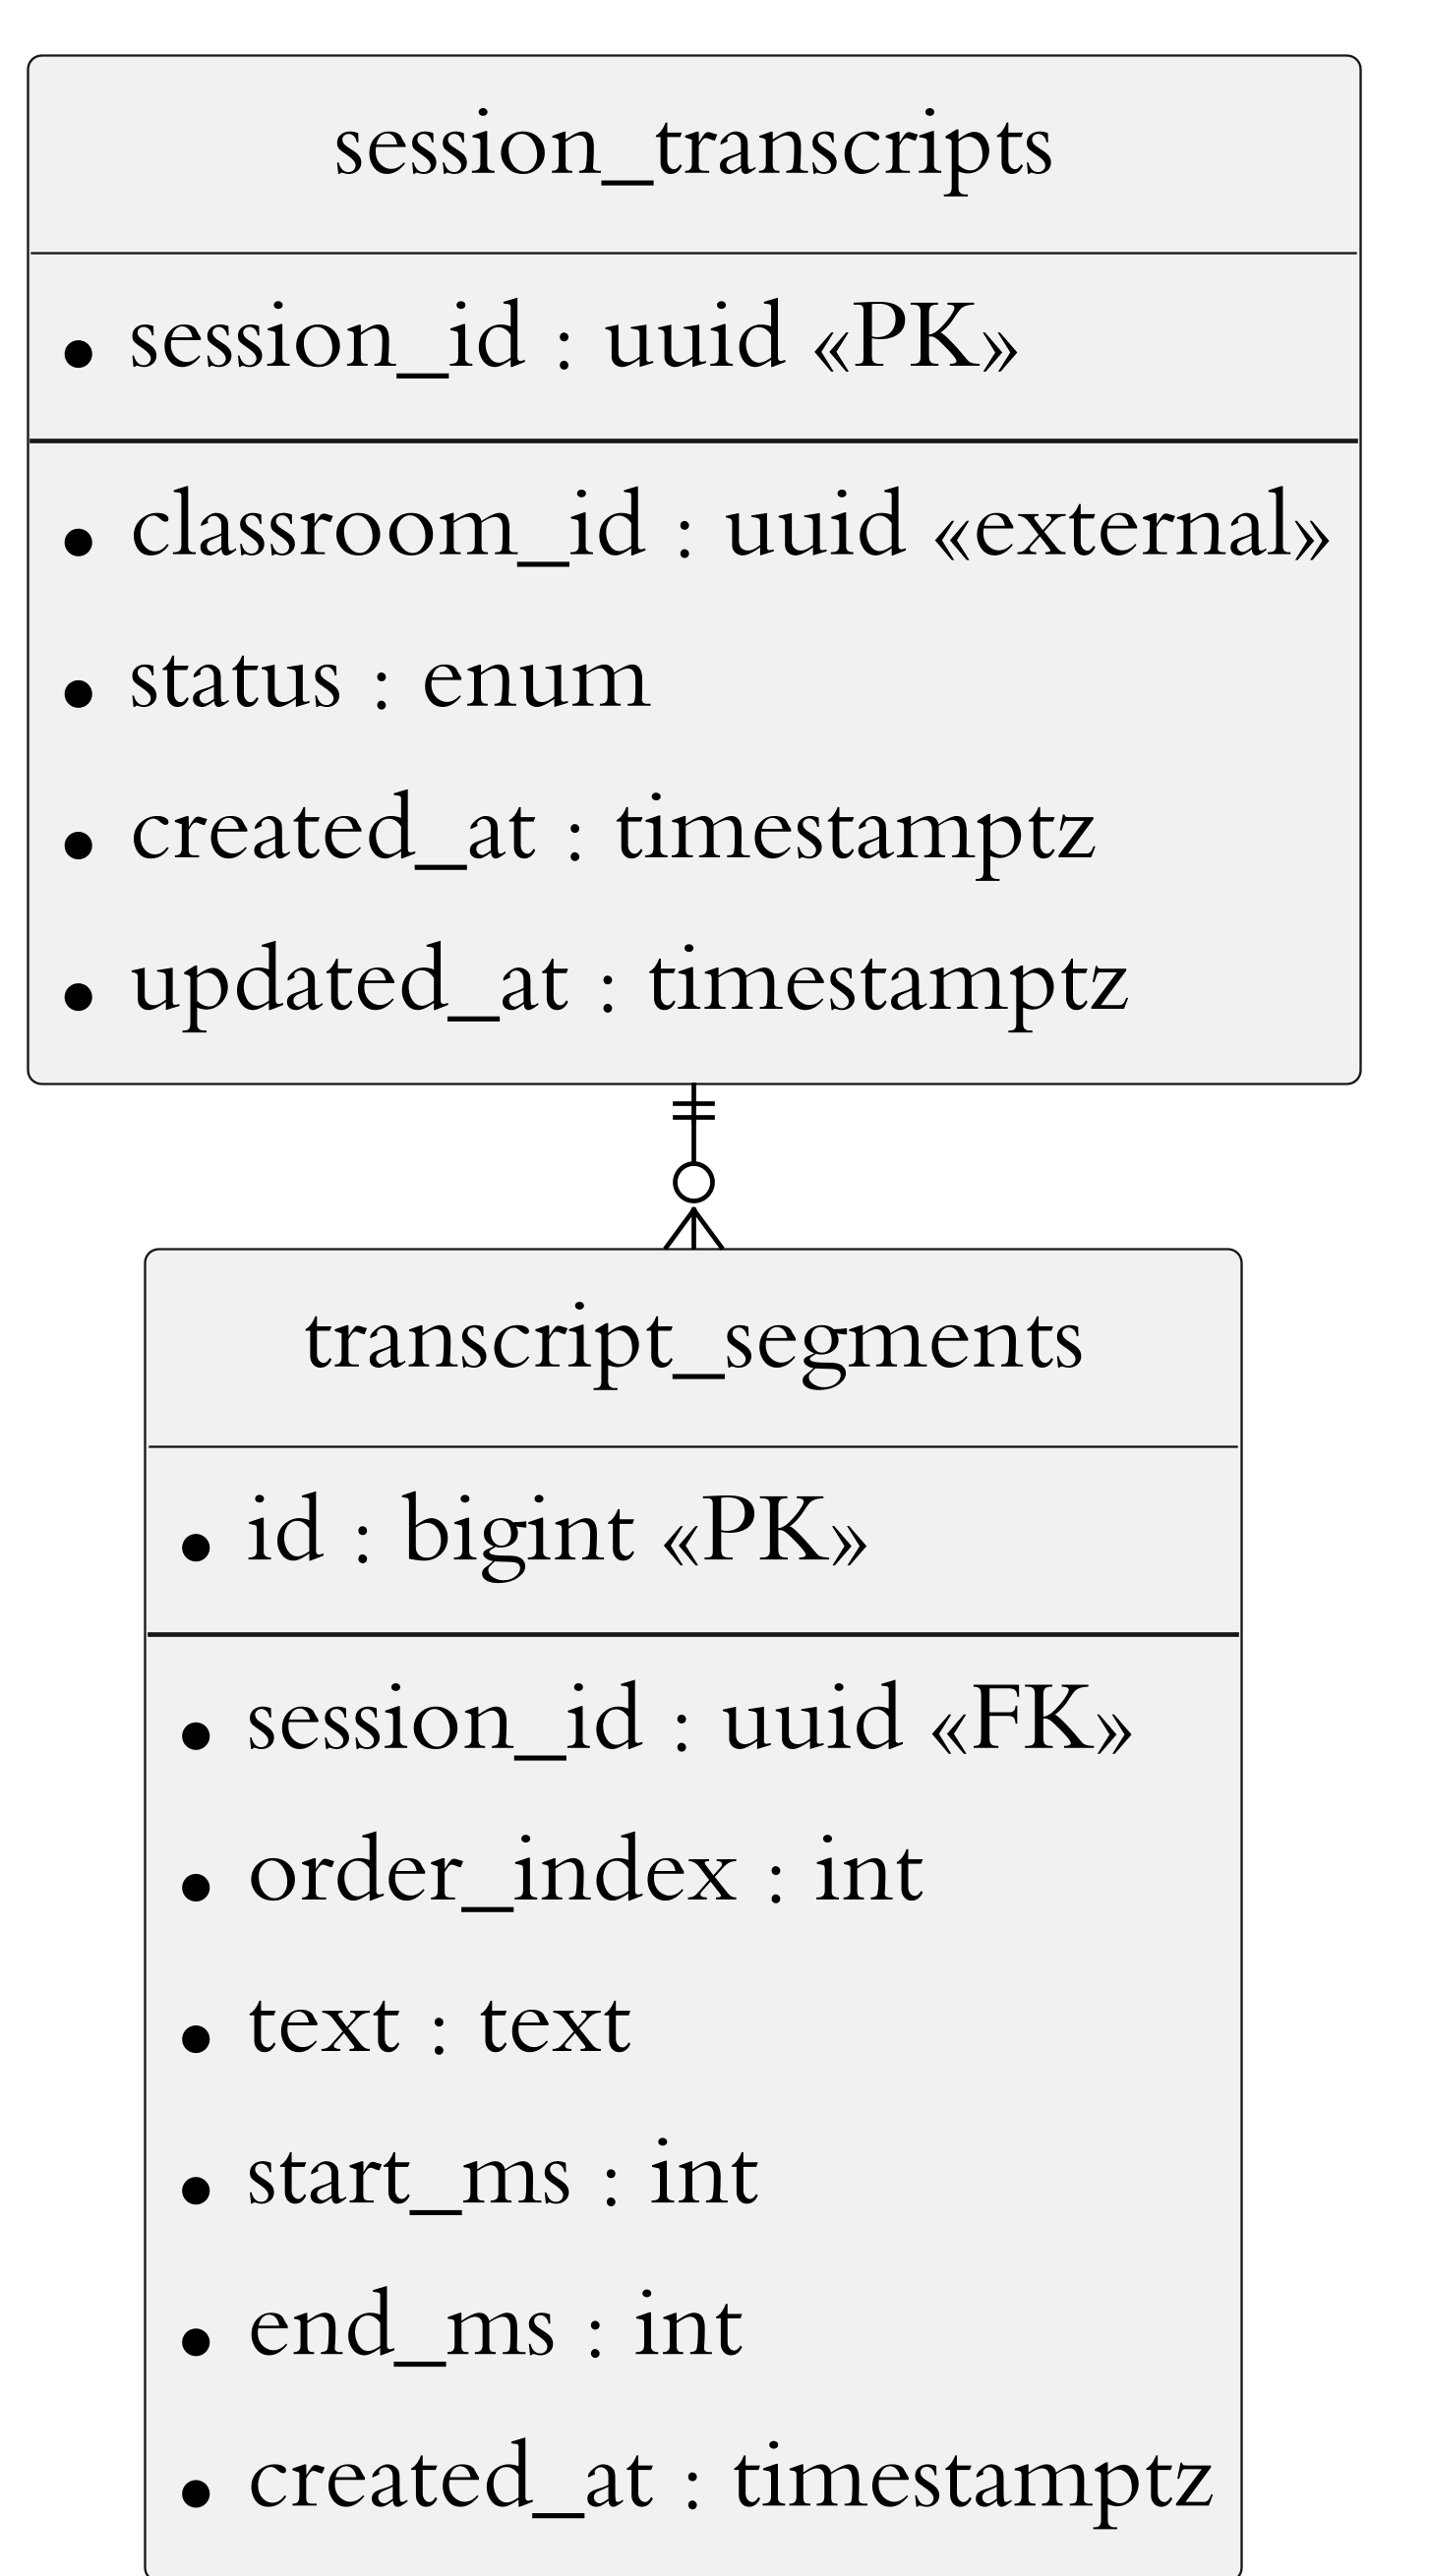
\includegraphics[width=\textwidth,height=0.8\textheight,keepaspectratio]{figures/erd-05-live-assistant.png}
  \caption{مخطط الكيانات والعلاقات لخدمة المساعد المباشر.}
  \label{fig:erd-05}
\end{figure}

ويضبط قيدُ فرادة مركّب على الزوج (\en{session\_id}, \en{order\_index}) تسلسلَ المقاطع داخل الجلسة ويمنع تكرار الرقم نفسه، في حين يؤدّي حذف الترويسة إلى حذف مقاطعها تتابعيًّا.
